% !TeX program = lualatex
\documentclass[UTF8,zihao=5,fontset=fandol,letterpaper]{ctexart}

\usepackage[hmargin=0.72in,vmargin=0.62in]{geometry}
\usepackage{graphicx}
\usepackage{enumitem}
\usepackage{titlesec}
\usepackage{xcolor}
\usepackage[hidelinks]{hyperref}

\pagestyle{empty}
\linespread{1.10}
\setlength{\parindent}{0pt}
\setlength{\parskip}{0pt}
\setlist{leftmargin=*,topsep=2pt,itemsep=3pt,parsep=0pt}
\titleformat{\section}{\large\bfseries}{}{0pt}{}[\vspace{2pt}\titlerule]
\titlespacing*{\section}{0pt}{8pt}{4pt}
\hypersetup{pdftitle={张哲畅个人简历},pdfauthor={张哲畅}}

\newcommand{\cvlink}[2]{\href{#1}{\underline{#2}}}
\newcommand{\publicationref}[2]{\mbox{\hyperref[#1]{#2 \underline{[\ref*{#1}]}}}}
\newcommand{\ccfa}{\mbox{\textcolor{red}{\textbf{(CCF-A)}}}}

\begin{document}

\begin{minipage}[t]{0.78\textwidth}
  \vspace{0pt}
  {\zihao{2}\bfseries 张哲畅}\\[4pt]
  信息学（Informatics）博士在读\\
  \begin{tabular}[t]{@{}l@{\hspace{0.8em}}l@{}}
    宾夕法尼亚州立大学 & {\small The Pennsylvania State University}\\
    信息科学与技术学院 & {\small College of Information Sciences and Technology}
  \end{tabular}\\
  {\small
    \href{mailto:zhechang@psu.edu}{\textcolor{blue!35!black}{zhechang@psu.edu}}
    \quad
    \href{https://1ncande5cence.github.io/}{\textcolor{blue!35!black}{1ncande5cence.github.io}}\\
    E338 Westgate Building, 288 Burrowes Rd, University Park, PA 16802, USA
  }
\end{minipage}\hfill
\begin{minipage}[t]{32mm}
  \vspace{0pt}
  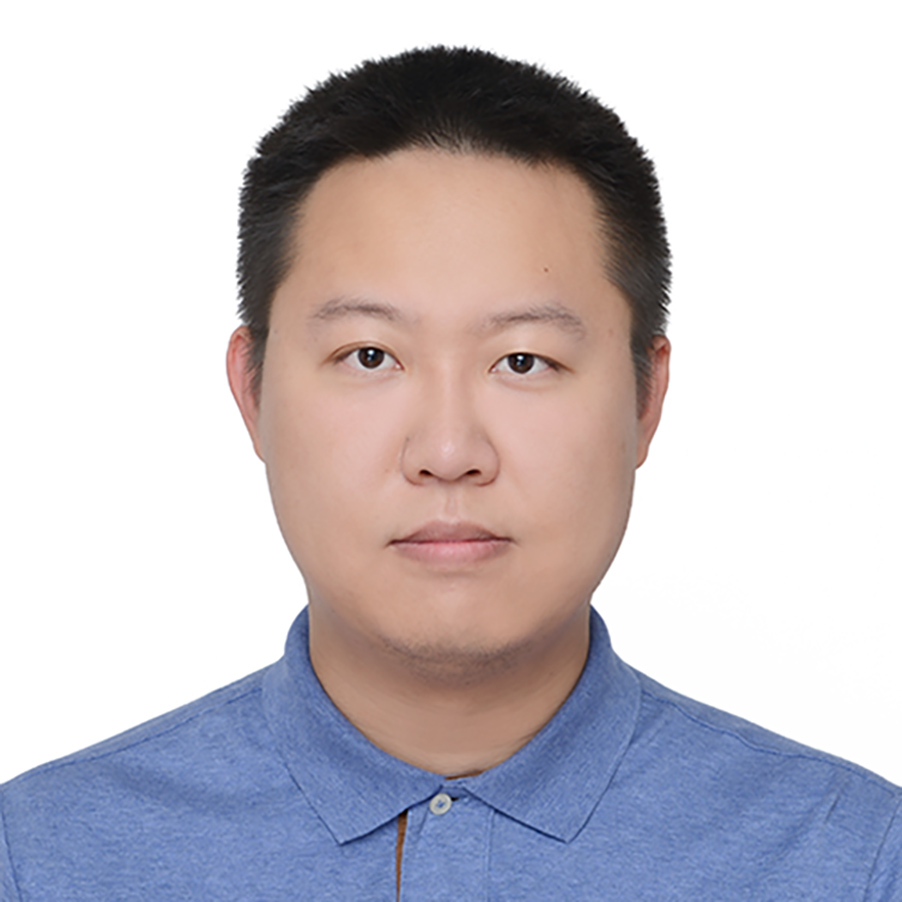
\includegraphics[width=\linewidth]{portrait_zh.jpg}
\end{minipage}

\section{研究方向}

我的研究方向是系统与软件安全（systems and software security），结合程序分析（program analysis）与大语言模型（LLMs）提取与安全相关的程序行为。研究工作涵盖漏洞利用生成（exploit generation）、防护机制评估、关键数据识别（critical data identification）和 AI 智能体系统安全。

\section{教育背景}

\begin{itemize}
  \item \textbf{宾夕法尼亚州立大学}，信息学（Informatics）博士在读
    \hfill 2023年8月--至今\\
    GPA 3.97/4.00，导师 \cvlink{https://huhong789.github.io/}{Hong Hu}\\
    开题题目：Leveraging High-Level Semantics for Exploit Generation and Defense Assessment
  \item \textbf{华中科技大学}，软件安全，工学硕士
    \hfill 2020年9月--2023年6月\\
    GPA 3.77/4.00（85.95/100），导师
    \cvlink{http://faculty.hust.edu.cn/zoudeqing/en/index.htm}{邹德清}、
    \cvlink{http://faculty.hust.edu.cn/yuanbin12/en/index.htm}{袁斌}\\
    学位论文：深度报文检测系统的漏洞挖掘研究
  \item \textbf{华中科技大学}，信息安全，工学学士
    \hfill 2016年9月--2020年6月\\
    GPA 3.95/4.00（90.7/100，排名 1/78）\\
    学位论文：面向基于特征的网络入侵检测系统的模糊测试
\end{itemize}

\section{工作经历}

\begin{itemize}
  \item \textbf{研究助理}，宾夕法尼亚州立大学（导师 \cvlink{https://huhong789.github.io/}{Hong Hu}）
    \hfill 2023年8月--至今
  \item \textbf{研究助理}，上海交通大学（导师 \cvlink{https://lijuanru.com/}{李卷孺}）
    \hfill 2019年6月--2019年8月
\end{itemize}

\section{同行评审会议论文}

\begin{enumerate}[label={[\arabic*]},ref=\arabic*]
  \raggedright
  \item\label{pub:contractguard}
    Hengkai Ye\textsuperscript{*}, \textbf{Zhechang Zhang}\textsuperscript{*}, Ruibo Lu, Jinyuan Jia, and Hong Hu.
    ContractGuard: Auditing Semantic Contracts of MCP Tools for Security Violations.
    \textit{CCS 2026}, The Hague, Netherlands, November 2026.
    \ccfa~\cvlink{https://www.sigsac.org/ccs/CCS2026/program/accepted-papers.html}{[Link]}
  \item\label{pub:sack}
    \textbf{Zhechang Zhang}, Hengkai Ye, Song Liu, and Hong Hu.
    SACK: Systematic Generation of Function Substitution Attacks Against Control-Flow Integrity.
    \textit{NDSS 2026}, San Diego, CA, USA, February 2026.
    \ccfa~\cvlink{https://www.ndss-symposium.org/ndss-paper/sack-systematic-generation-of-function-substitution-attacks-against-control-flow-integrity/}{[Link]}
  \item\label{pub:countdown}
    Shuangpeng Bai, \textbf{Zhechang Zhang}, and Hong Hu.
    CountDown: Refcount-guided Fuzzing for Exposing Temporal Memory Errors in Linux Kernel.
    \textit{CCS 2024}, Salt Lake City, UT, USA, October 2024.
    \ccfa~\cvlink{https://dl.acm.org/doi/10.1145/3658644.3690320}{[Link]}
  \item\label{pub:viper}
    Hengkai Ye, Song Liu, \textbf{Zhechang Zhang}, and Hong Hu.
    VIPER: Spotting Syscall-Guard Variables for Data-Only Attacks.
    \textit{USENIX Security 2023}, Anaheim, CA, USA, August 2023.
    \ccfa~\cvlink{https://www.usenix.org/system/files/usenixsecurity23-ye.pdf}{[Link]}
  \item\label{pub:statediver}
    \textbf{Zhechang Zhang}, Bin Yuan, Kehan Yang, Deqing Zou, and Hai Jin.
    StateDiver: Testing Deep Packet Inspection Systems with State-Discrepancy Guidance.
    \textit{ACSAC 2022}, Austin, TX, USA, December 2022.
    \mbox{\textbf{(CCF-B)}}~\cvlink{https://doi.org/10.1145/3564625.3564650}{[Link]}
\end{enumerate}
\textsuperscript{*} 共同第一作者.

\newpage
\section{学术海报与工业界会议}

\begin{itemize}
  \raggedright
  \item \textbf{Zhechang Zhang} and Hong Hu.
    How Close Are We? Measuring the Gap Between Dynamically and Statically Identified Indirect-Call Targets.
    (Poster) \textit{USENIX Security 2026}, Baltimore, MD, USA, August 2026.
    \cvlink{https://www.usenix.org/conference/usenixsecurity26/poster-session}{[Link]}
  \item Hengkai Ye, Song Liu, \textbf{Zhechang Zhang}, and Hong Hu.
    One Flip is All It Takes.
    (Industry Talk) \textit{Black Hat Asia Briefings 2024}, Singapore, April 2024.
    \cvlink{https://www.blackhat.com/asia-24/briefings/schedule/index.html\#one-flip-is-all-it-takes-identifying-syscall-guard-variables-for-data-only-attacks-36285}{[Link]}
\end{itemize}

\section{荣誉与奖励}

\begin{itemize}
  \item \textbf{春季学术差旅奖学金（Spring Travel Award）}，宾夕法尼亚州立大学信息科学与技术学院，2026年
  \item \textbf{优秀毕业生}，华中科技大学，2023年、2020年
  \item \textbf{国家奖学金}（0.1\%），2022年、2018年
  \item \textbf{第十七届“挑战杯”揭榜挂帅专项赛特等奖,擂主}（1/32），2022年
  \item \textbf{本科特优生}（1\%），华中科技大学，2018年
\end{itemize}

\section{学术服务与教学}

\textbf{外部审稿人（External Reviewer）}
\begin{itemize}
  \item USENIX Security Symposium（USENIX Security）\hfill 2025、2026年
  \item Network and Distributed System Security Symposium（NDSS）\hfill 2024--2026年
  \item ACM Conference on Computer and Communications Security（CCS）\hfill 2024、2025年
  \item International Conference on Applied Cryptography and Network Security（ACNS）\hfill 2026年
  \item International Symposium on Research in Attacks, Intrusions and Defenses（RAID）\hfill 2026年
  \item IEEE Transactions on Dependable and Secure Computing（TDSC）\hfill 2023年
\end{itemize}

\smallskip
\textbf{程序委员会委员（Program Committee Member）}
\begin{itemize}
  \item IEEE International Conference on Parallel and Distributed Systems（ICPADS）\hfill 2026年
\end{itemize}

\smallskip
\textbf{课程助教（Teaching Assistant）}
\begin{itemize}
  \item 操作系统，华中科技大学\hfill 2019年秋季
\end{itemize}

\section{开源项目}

\begin{itemize}
  \raggedright
  \item \textbf{ContractGuard}：比对 MCP 工具的描述与实际实现的安全问题识别框架（\publicationref{pub:contractguard}{CCS 2026}）~
    \cvlink{https://github.com/PSU-Security-Universe/contractguard}{[源码]}
  \item \textbf{SACK}：自动生成控制流完整性（CFI）防护下的函数替换攻击框架（\publicationref{pub:sack}{NDSS 2026}）~
    \cvlink{https://github.com/PSU-Security-Universe/sack}{[源码]}
  \item \textbf{CountDown}：用引用计数（reference counts）引导的模糊测试工具（\publicationref{pub:countdown}{CCS 2024}）~
    \cvlink{https://github.com/PSU-Security-Universe/countdown}{[源码]}
  \item \textbf{VIPER}：自动化识别系统调用关键变量（syscall-guard variables）的分析工具\allowbreak
    （\publicationref{pub:viper}{USENIX Security 2023}）~
    \cvlink{https://github.com/PSU-Security-Universe/viper}{[源码]}
  \item \textbf{StateDiver}：利用状态差异引导深度报文检测（DPI）系统测试的框架（\publicationref{pub:statediver}{ACSAC 2022}）~
    \cvlink{https://github.com/CGCL-codes/StateDiver}{[源码]}
\end{itemize}

\section{漏洞发现}

\begin{tabular*}{\textwidth}{@{}l@{\extracolsep{\fill}}lll@{}}
  \textbf{CVE 编号} & \textbf{漏洞类型} & \textbf{受影响软件} & \textbf{受影响版本}\\[2pt]
  \cvlink{https://nvd.nist.gov/vuln/detail/CVE-2021-45098}{CVE-2021-45098} &
  解释冲突（Interpretation Conflict） & Suricata & 5.0.0--5.0.7、6.0.0--6.0.3
\end{tabular*}

\end{document}
